% CREATED BY DAVID FRISK, 2015
\chapter{Results}
Lorem ipsum dolor sit amet, consectetur adipisicing elit, sed do eiusmod tempor incididunt ut labore et dolore magna aliqua. Ut enim ad minim veniam, quis nostrud exercitation ullamco laboris nisi ut aliquip ex ea commodo consequat. Duis aute irure dolor in reprehenderit in voluptate velit esse cillum dolore eu fugiat nulla pariatur. Excepteur sint occaecat cupidatat non proident, sunt in culpa qui officia deserunt mollit anim id est laborum.




\section{Polar Geodesic coordinates}
\subsection{Visual Output}

\begin{figure}[H]
\centering
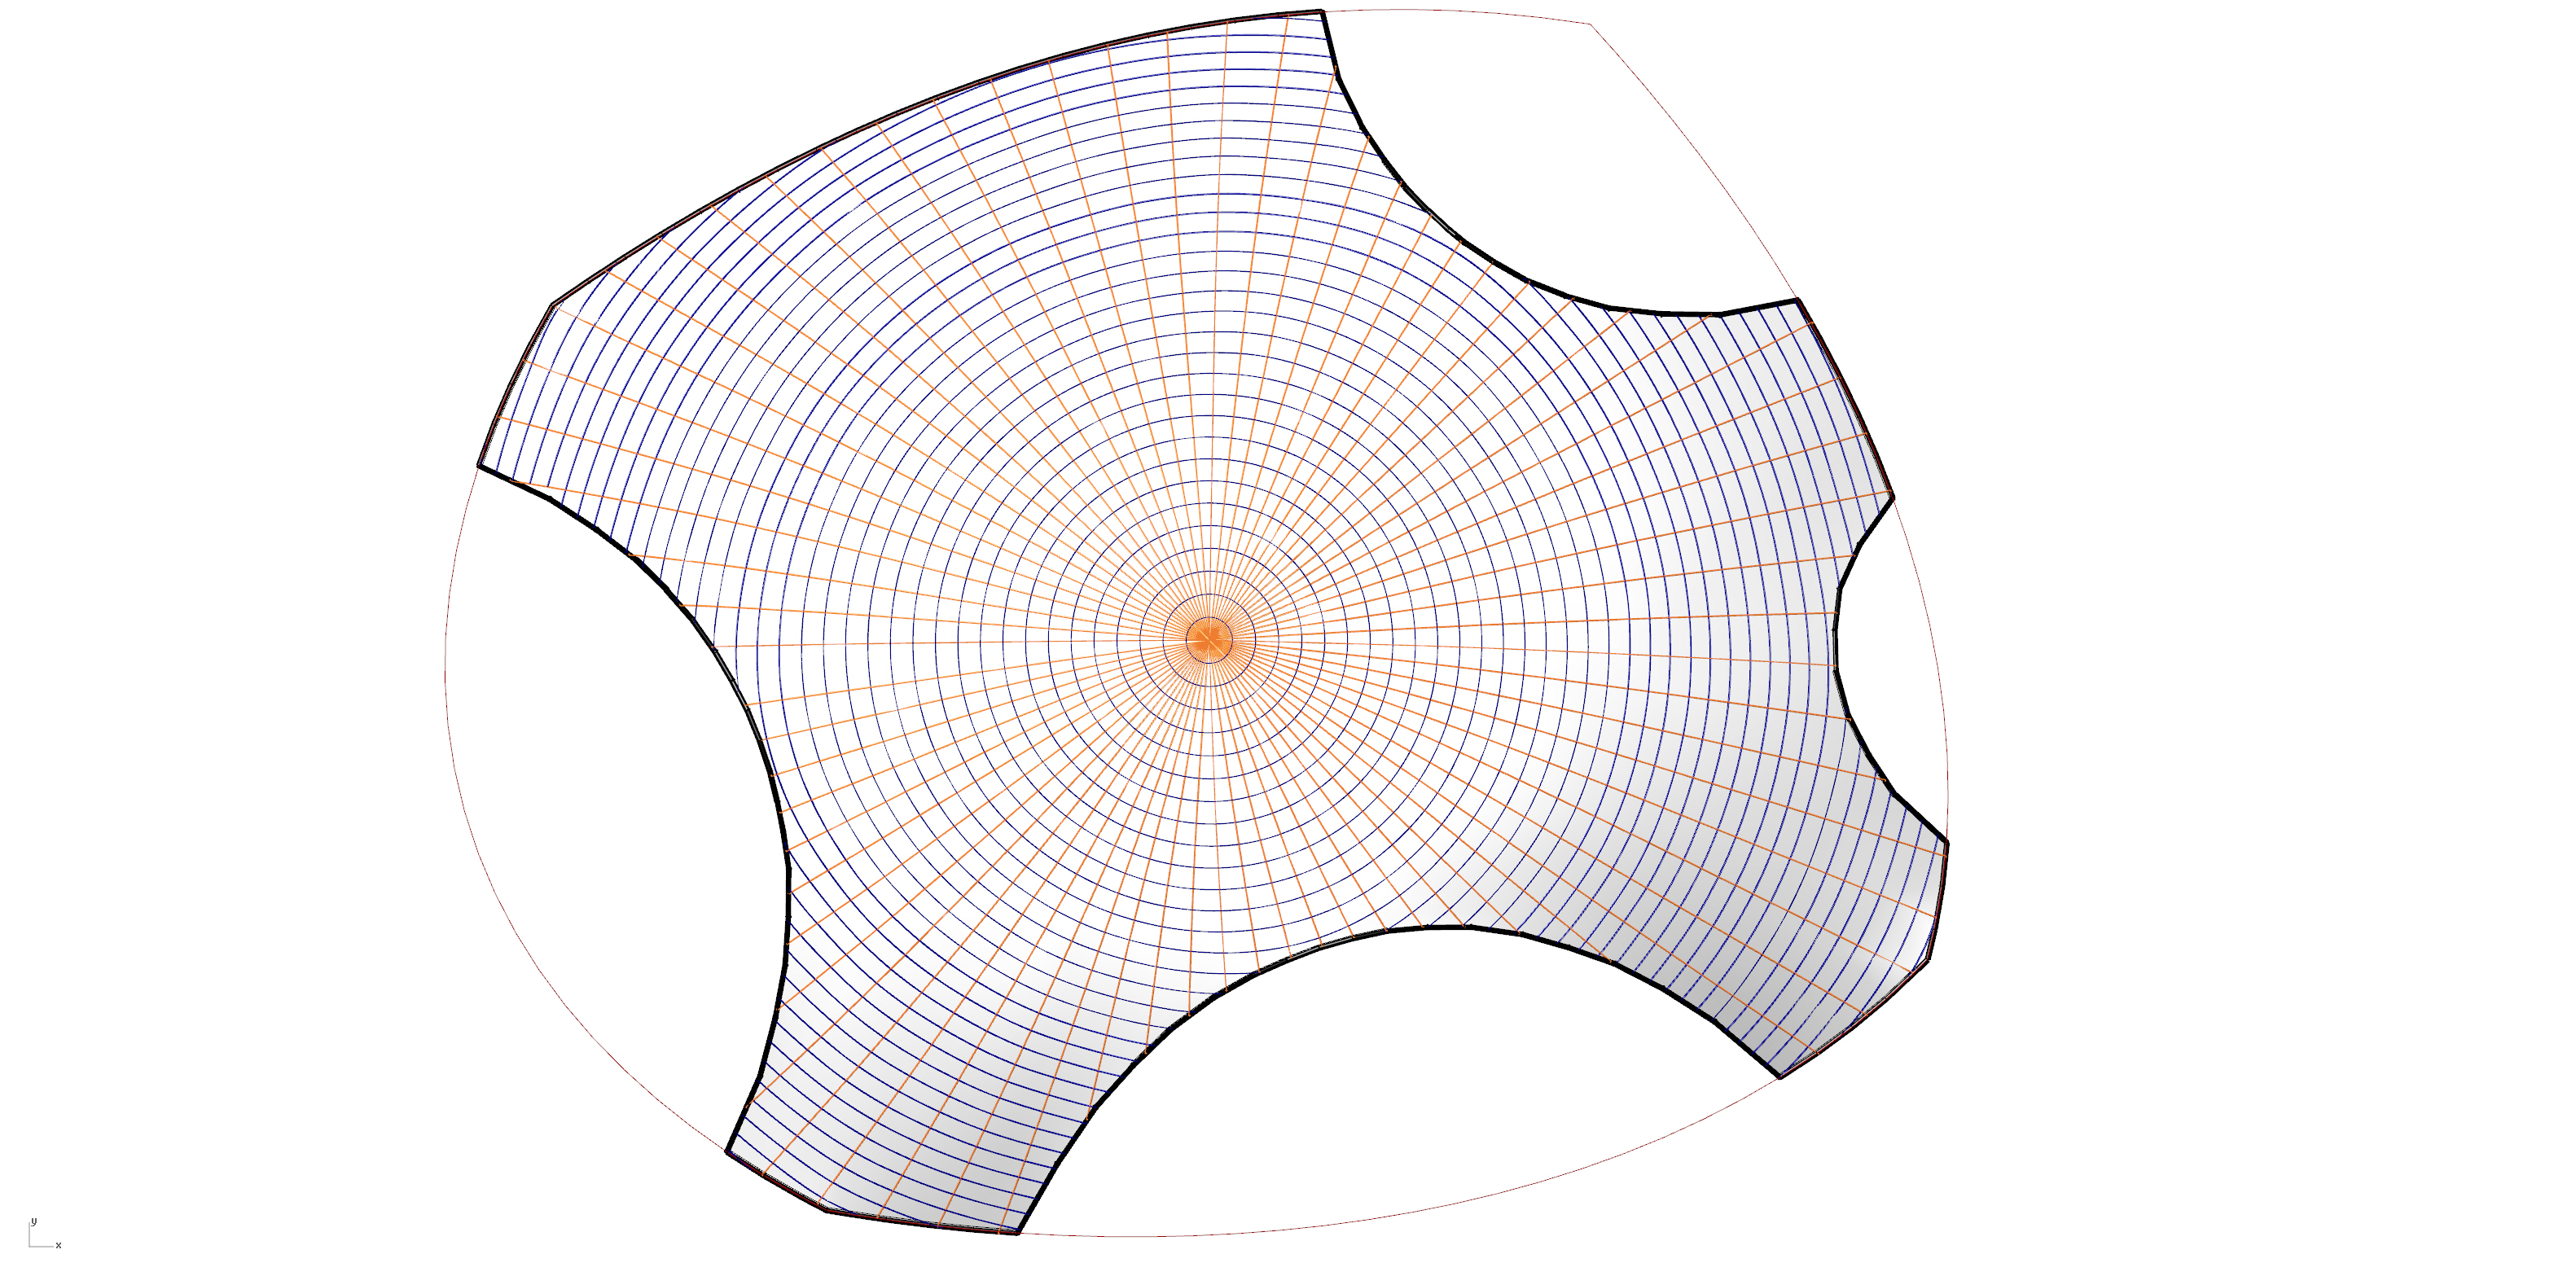
\includegraphics[width=1.0\linewidth ]{figure/Results/geotop2.jpg}
\caption{output from Geodesic}
\end{figure}

\begin{figure}[H]
\centering
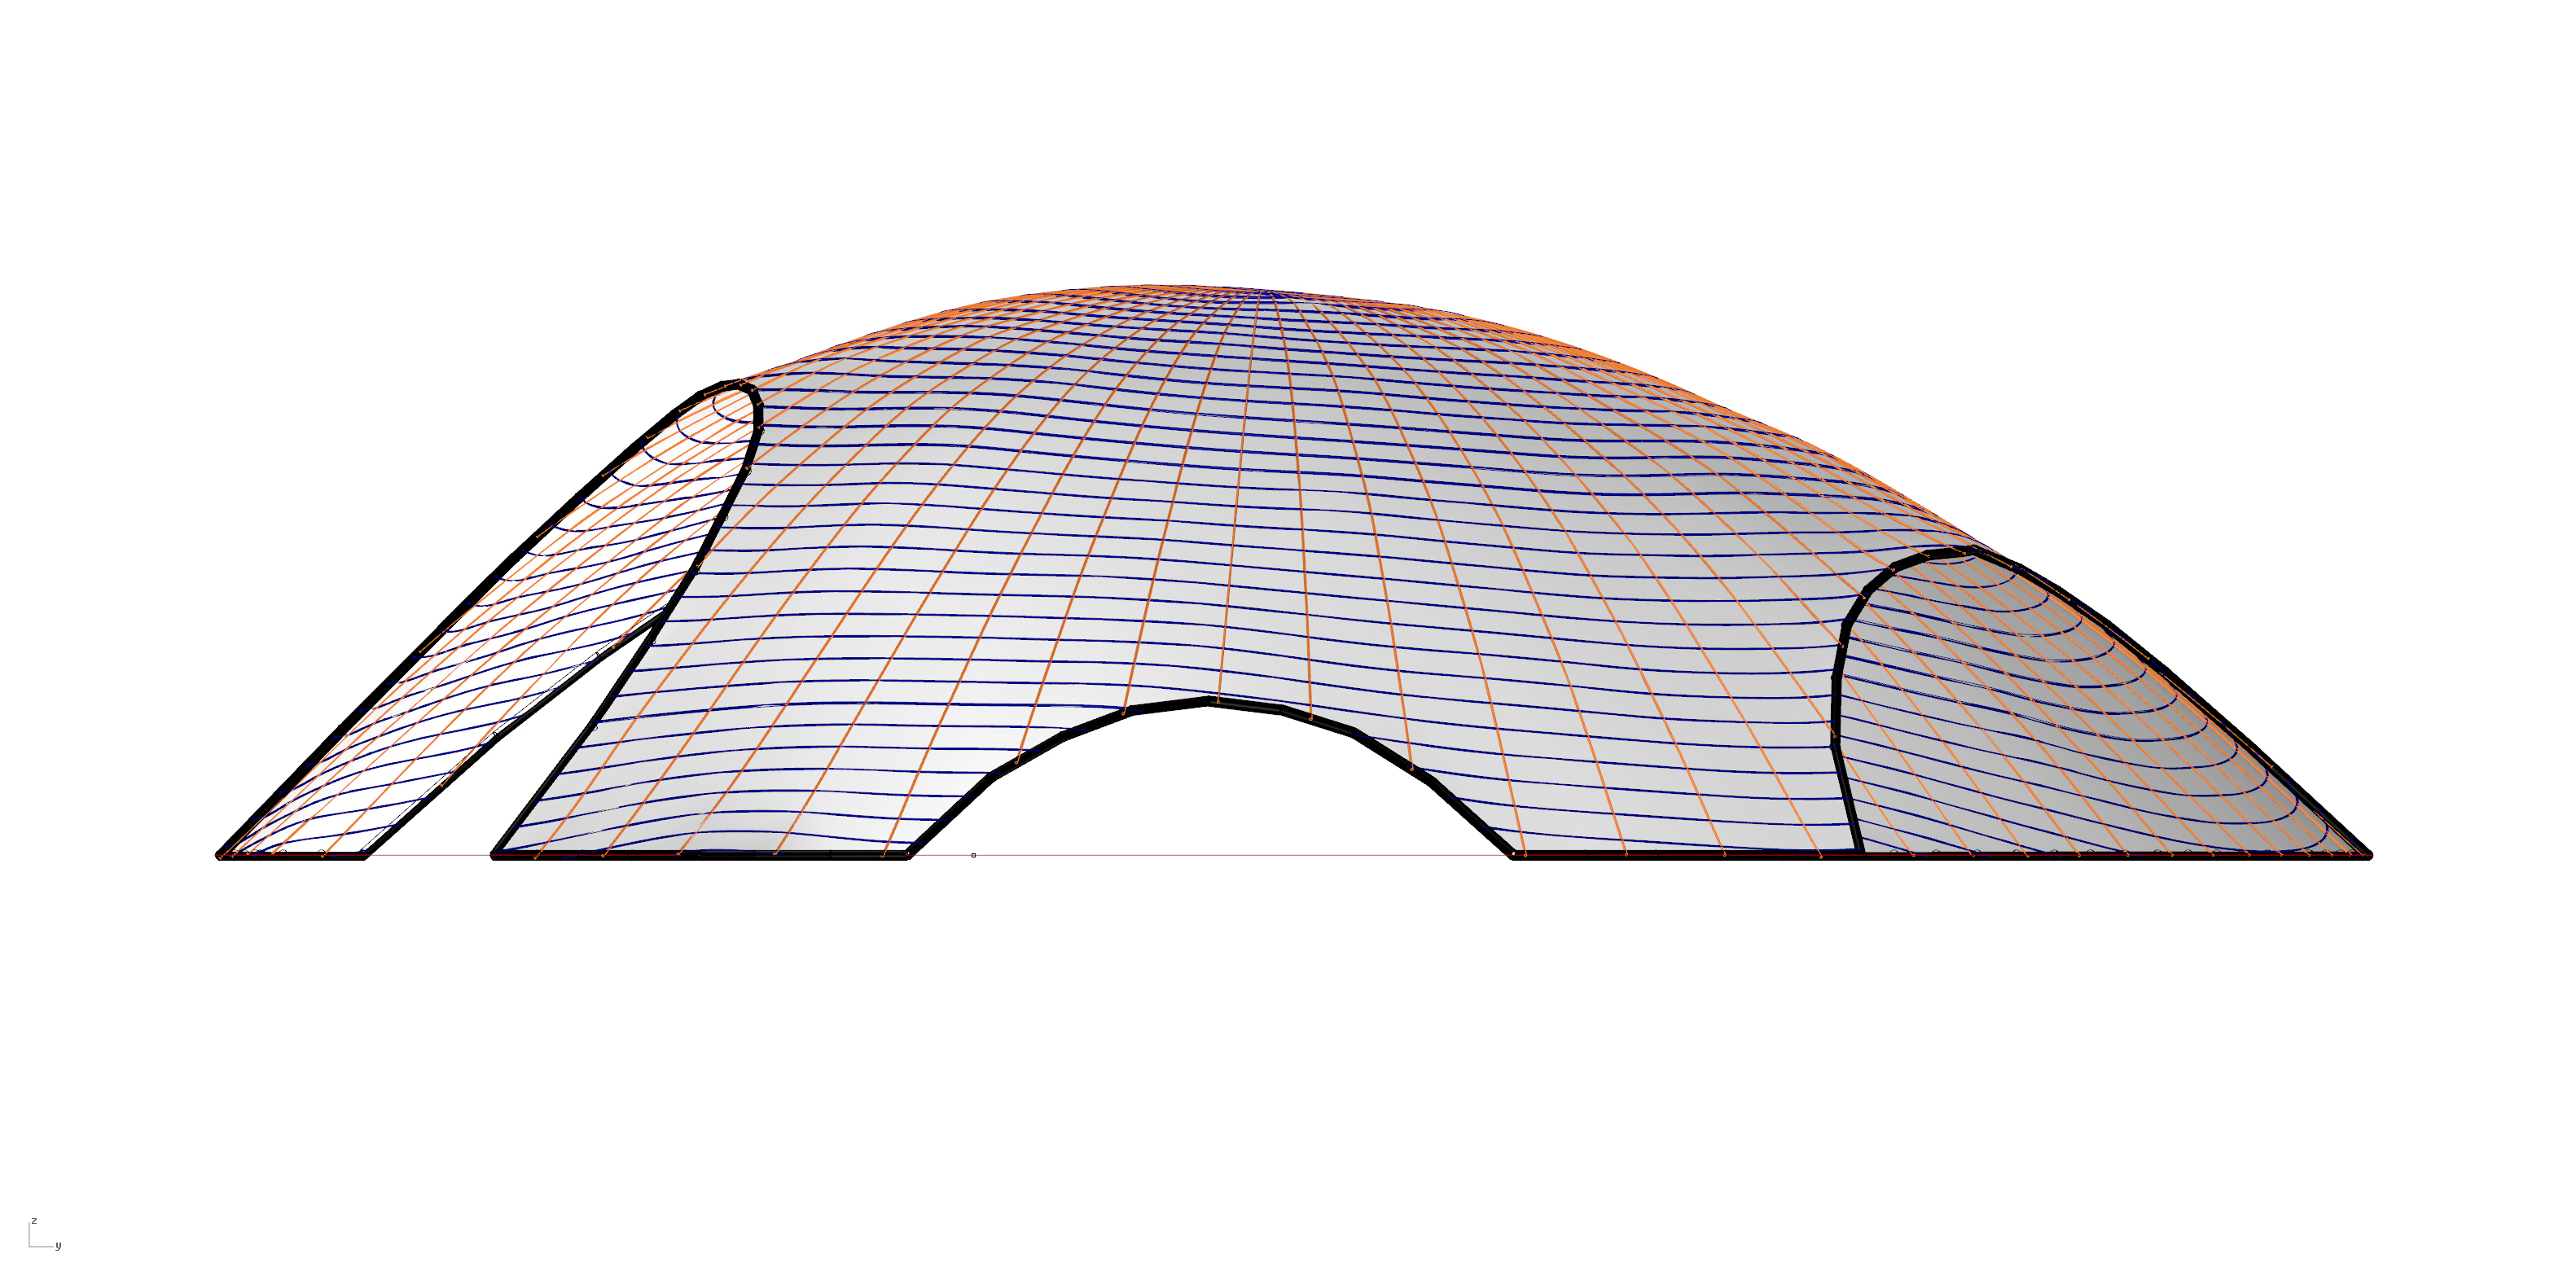
\includegraphics[width=1.0\linewidth ]{figure/Results/geoRight2.jpg}
\caption{output from Geodesic}
\end{figure}
\begin{figure}[H]
\centering
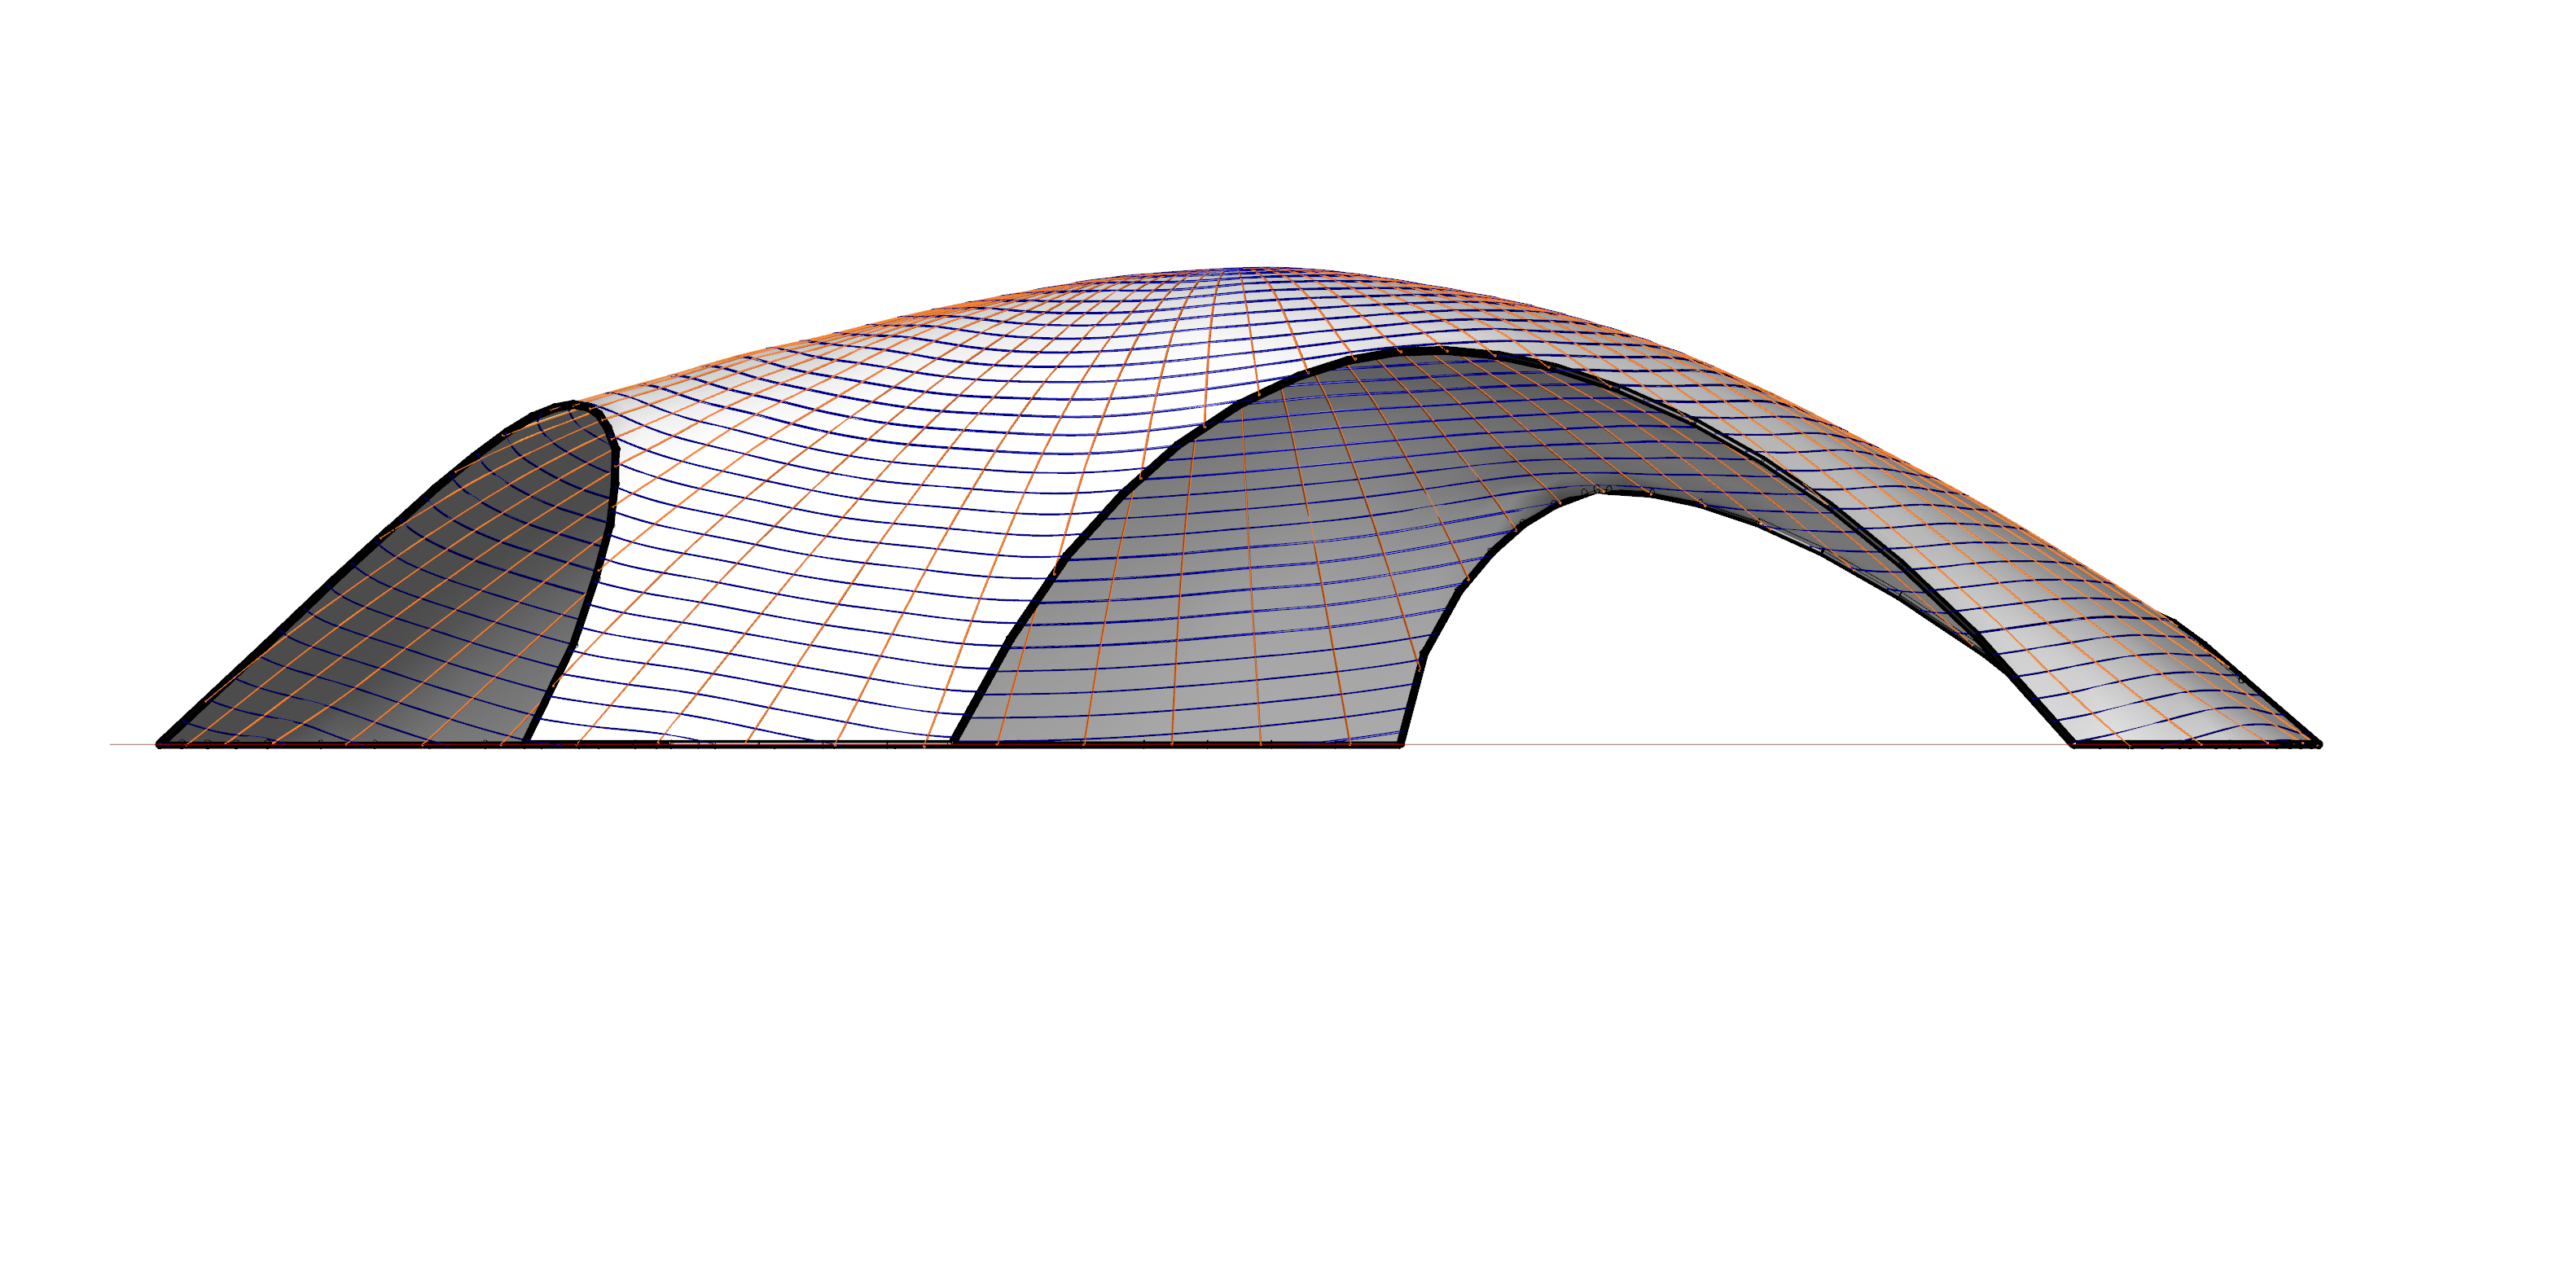
\includegraphics[width=1.0\linewidth ]{figure/Results/geofront2.jpg}
\caption{output from Geodesic}
\end{figure}
\begin{figure}[H]
\centering
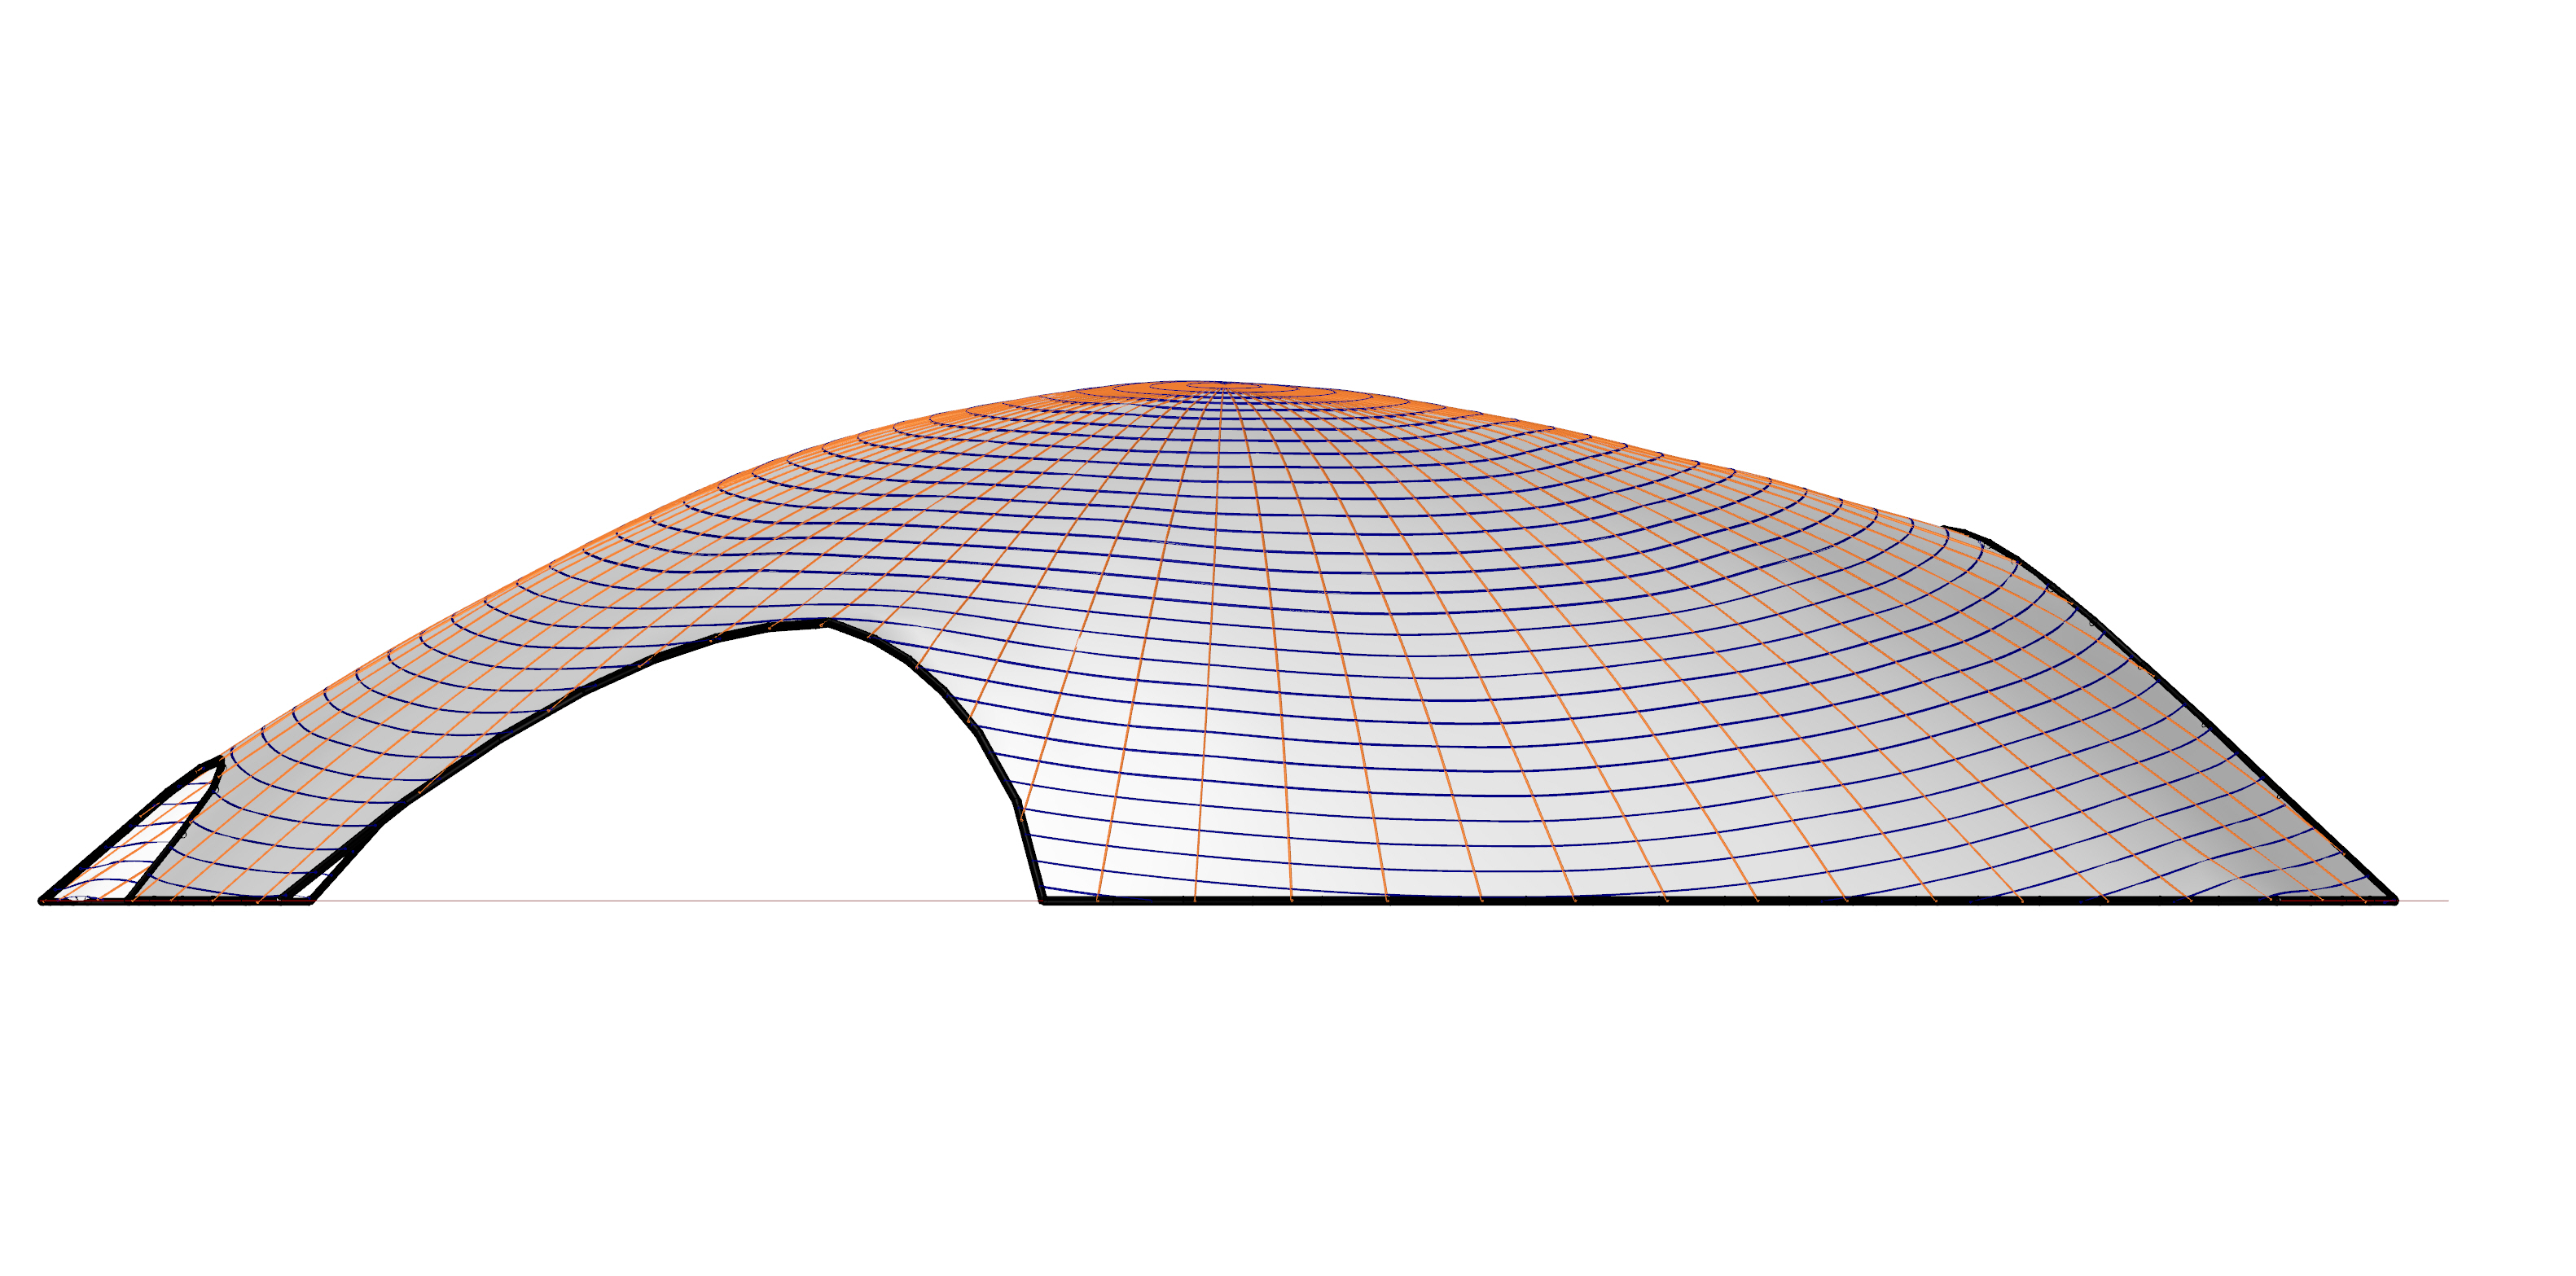
\includegraphics[width=1.0\linewidth ]{figure/Results/geoBack2.jpg}
\caption{output from Geodesic}
\end{figure}


\subsection{Geodesics}



\begin{figure}[H]
\centering
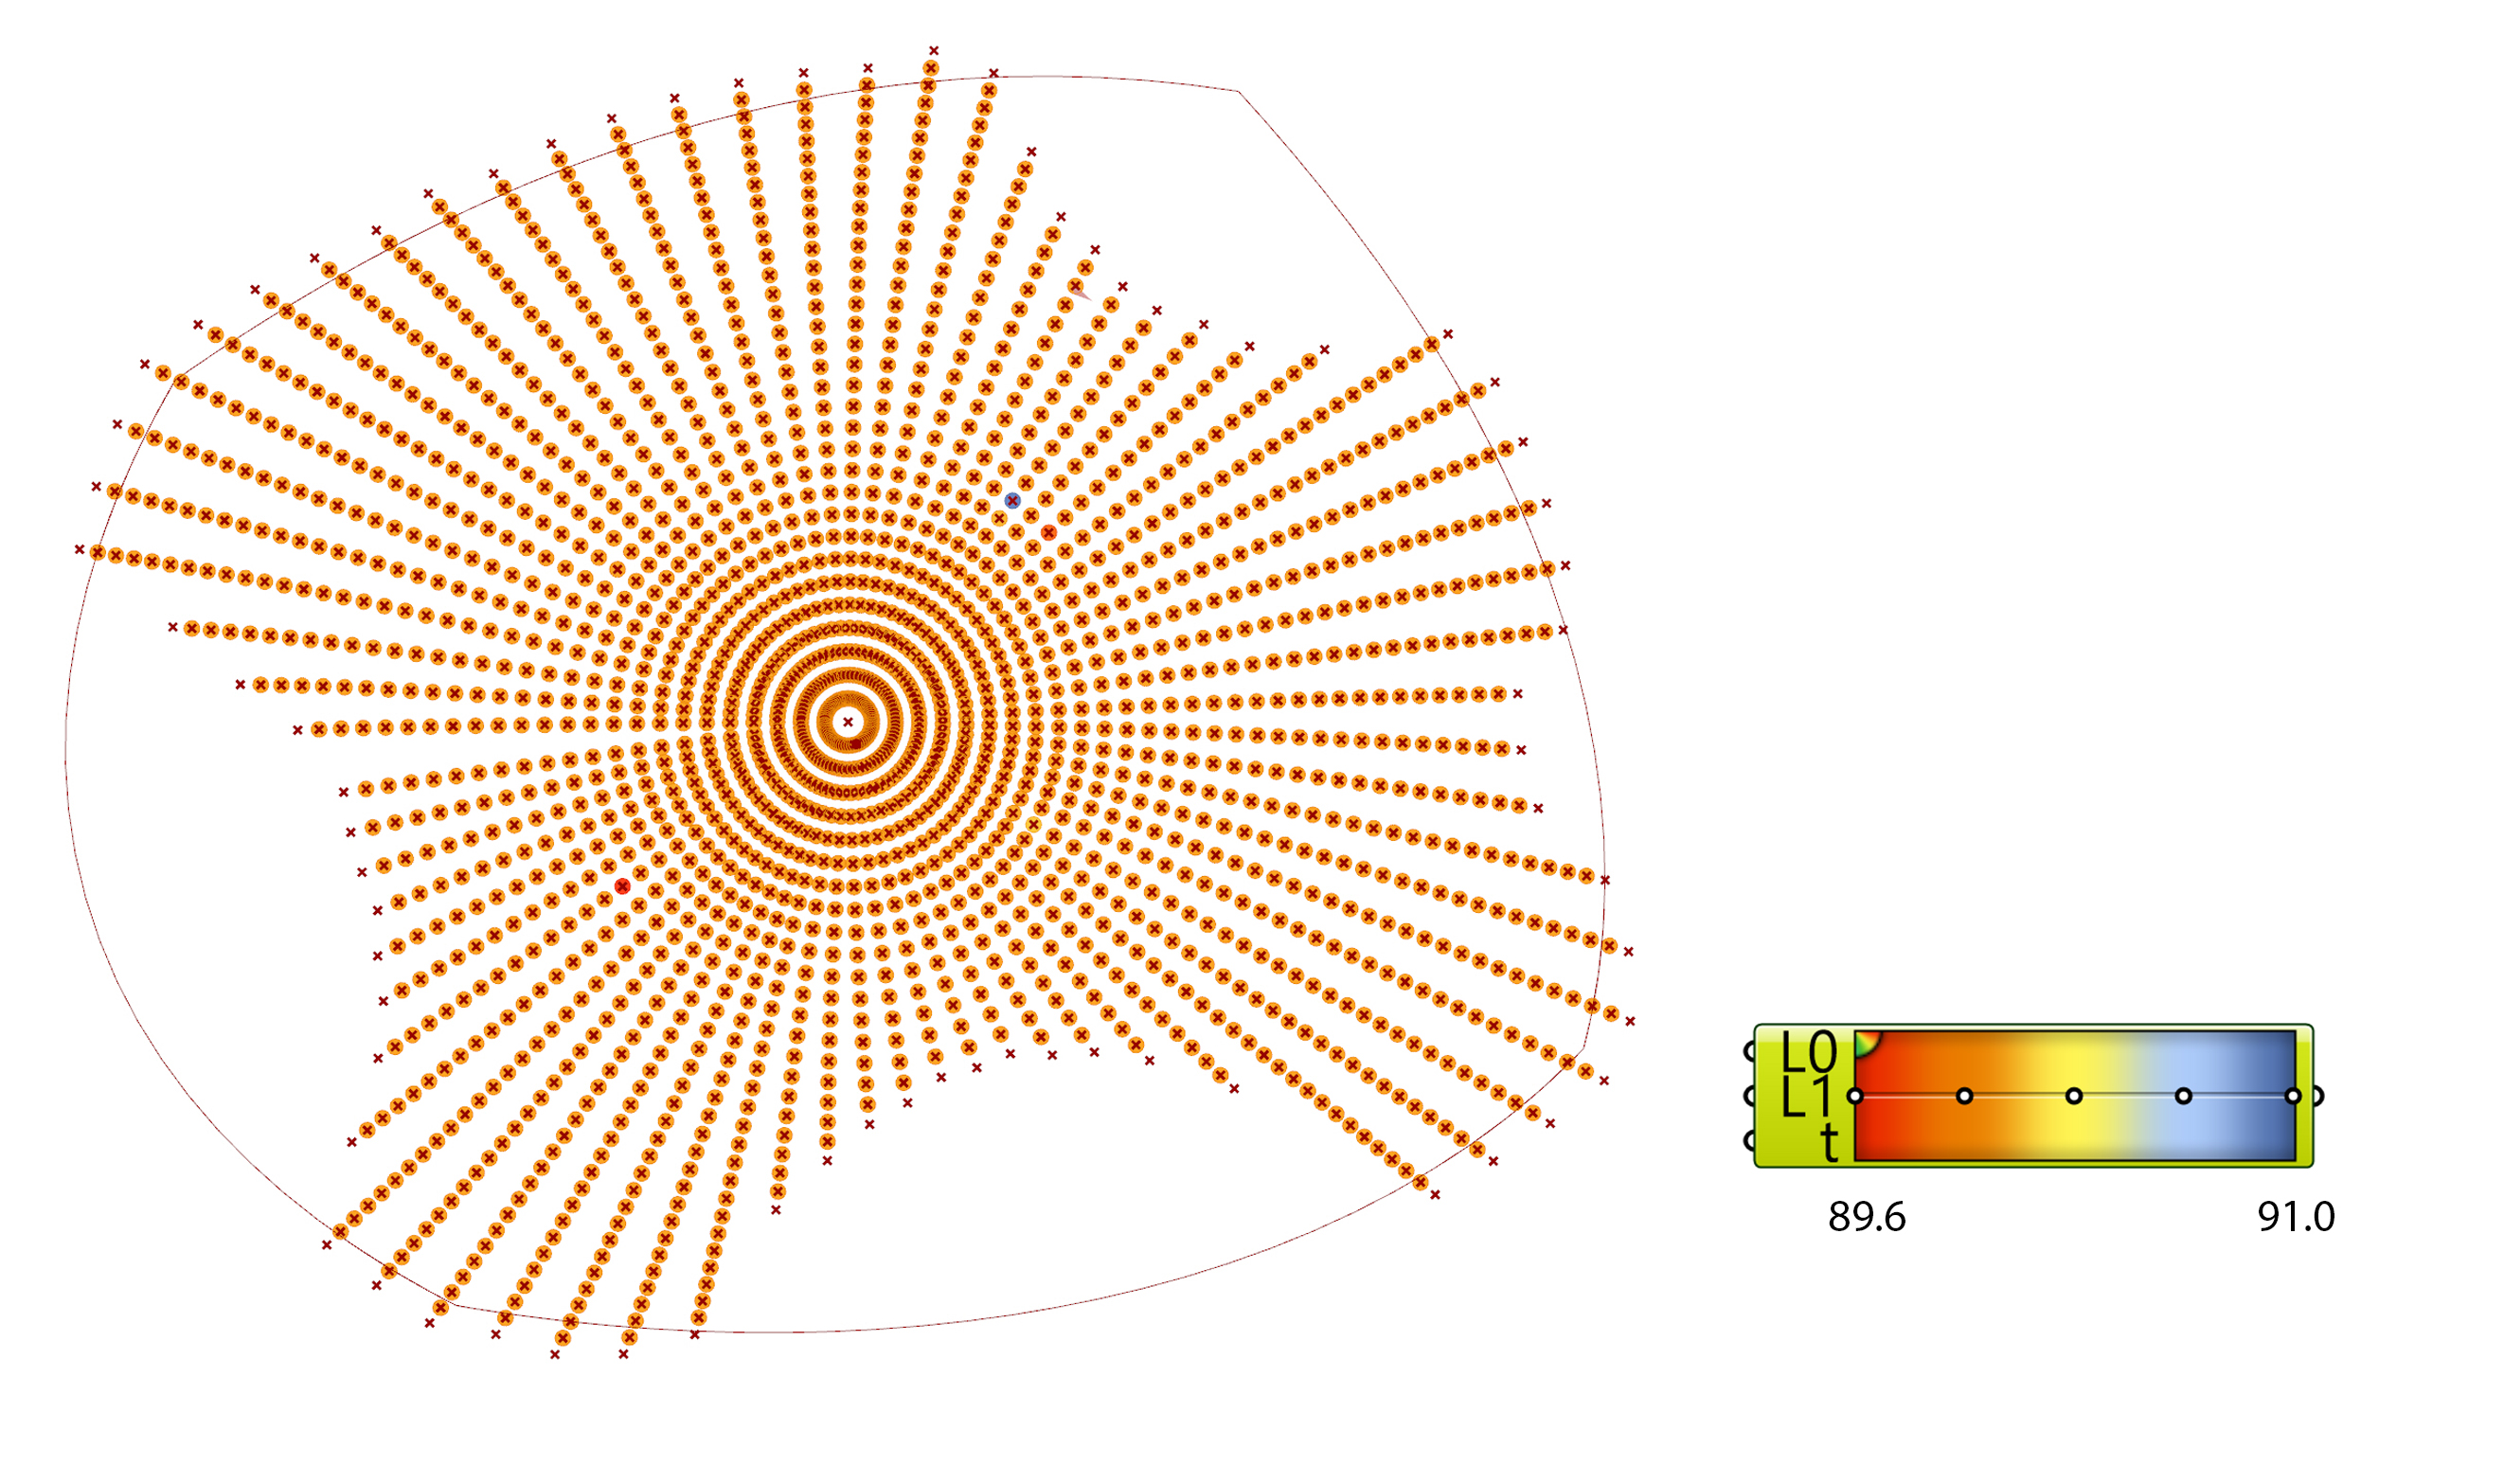
\includegraphics[width=1.0\linewidth ]{figure/Results/anglesdots2.jpg}
\caption{Graphical output of the angle between the normal and the cross product of the two connecting vectors to each point. }
\end{figure}

\begin{itemize}
    \item \textbf{Maximal Deviance of all geodesic sets: 0.97 \textdegree}\\
    This is the highest value of all geodesics pointsm, meaning that the deviance cannot be higher than this.
    \item \textbf{Average Deviance of the worst nodes in each geodesic set: 0.034 \textdegree}\\
    For each geodesic sets the nodes with highest deviance from 90 degrees was put together in a list. This measure is for those
    \item \textbf{Average Angle of all geodesic sets: 90.000 \textdegree}\\
    This is an average for all geodesic points in all geodesic set of points.
  
\end{itemize}


\begin{figure}[H]
\centering
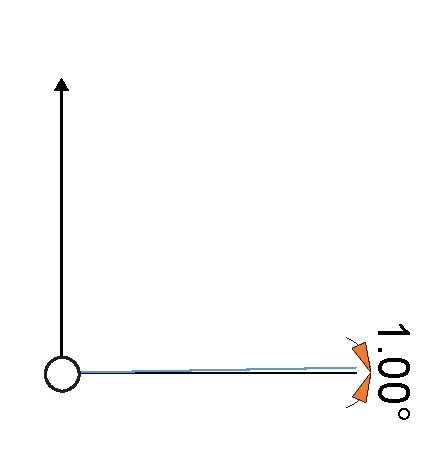
\includegraphics[width=0.6\linewidth ]{figure/Results/angle.pdf}
\caption{output from Geodesic}
\end{figure}

\subsection{Trajectories}

\begin{figure}[H]
\centering
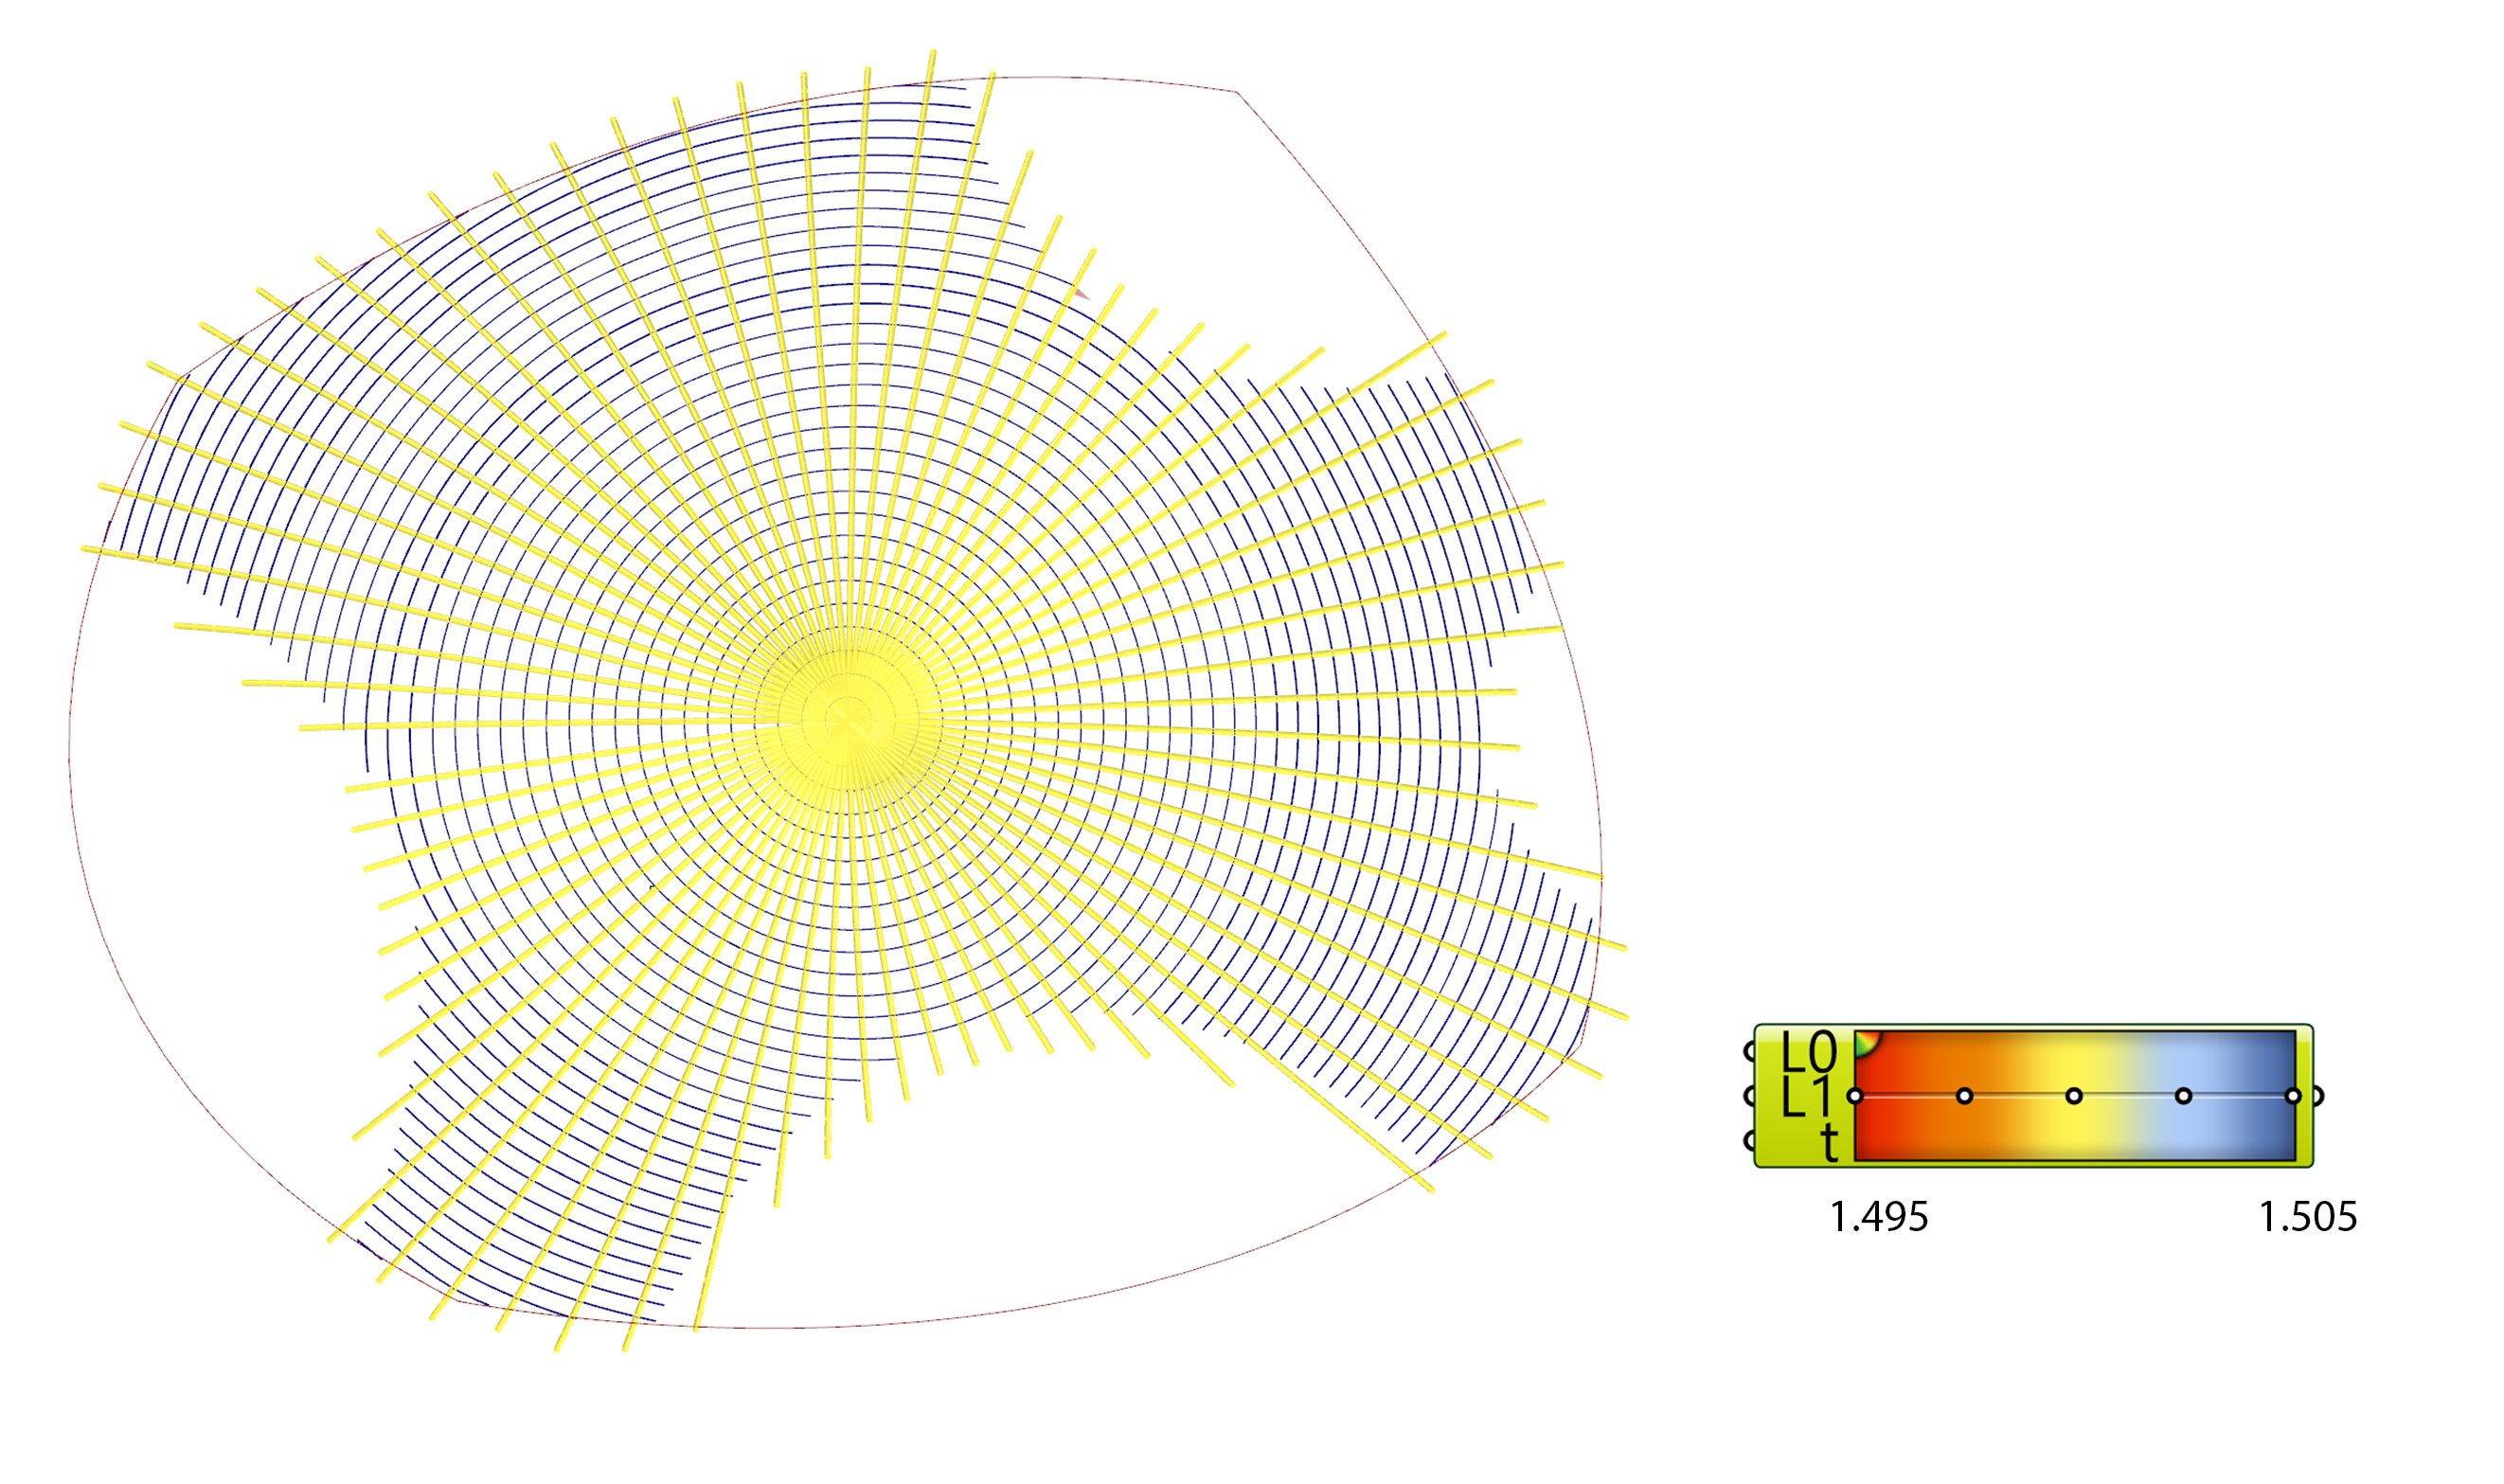
\includegraphics[width=1.0\linewidth ]{figure/Results/langthsgrad.jpg}
\caption{output from Geodesic}
\end{figure}


\begin{itemize}
    
    \item \textbf{Average geodesic segments: 1.499 units }\\
    This is an average for all geodesic points in all geodesic set of points.
    \item \textbf{maximal deviation from average segment segments:  0.0005 units }\\
    This is the maximal deviation of one segment compared to the average segment length
   

  
\end{itemize}







\section{Model preparation}



\begin{figure}[H]
\centering
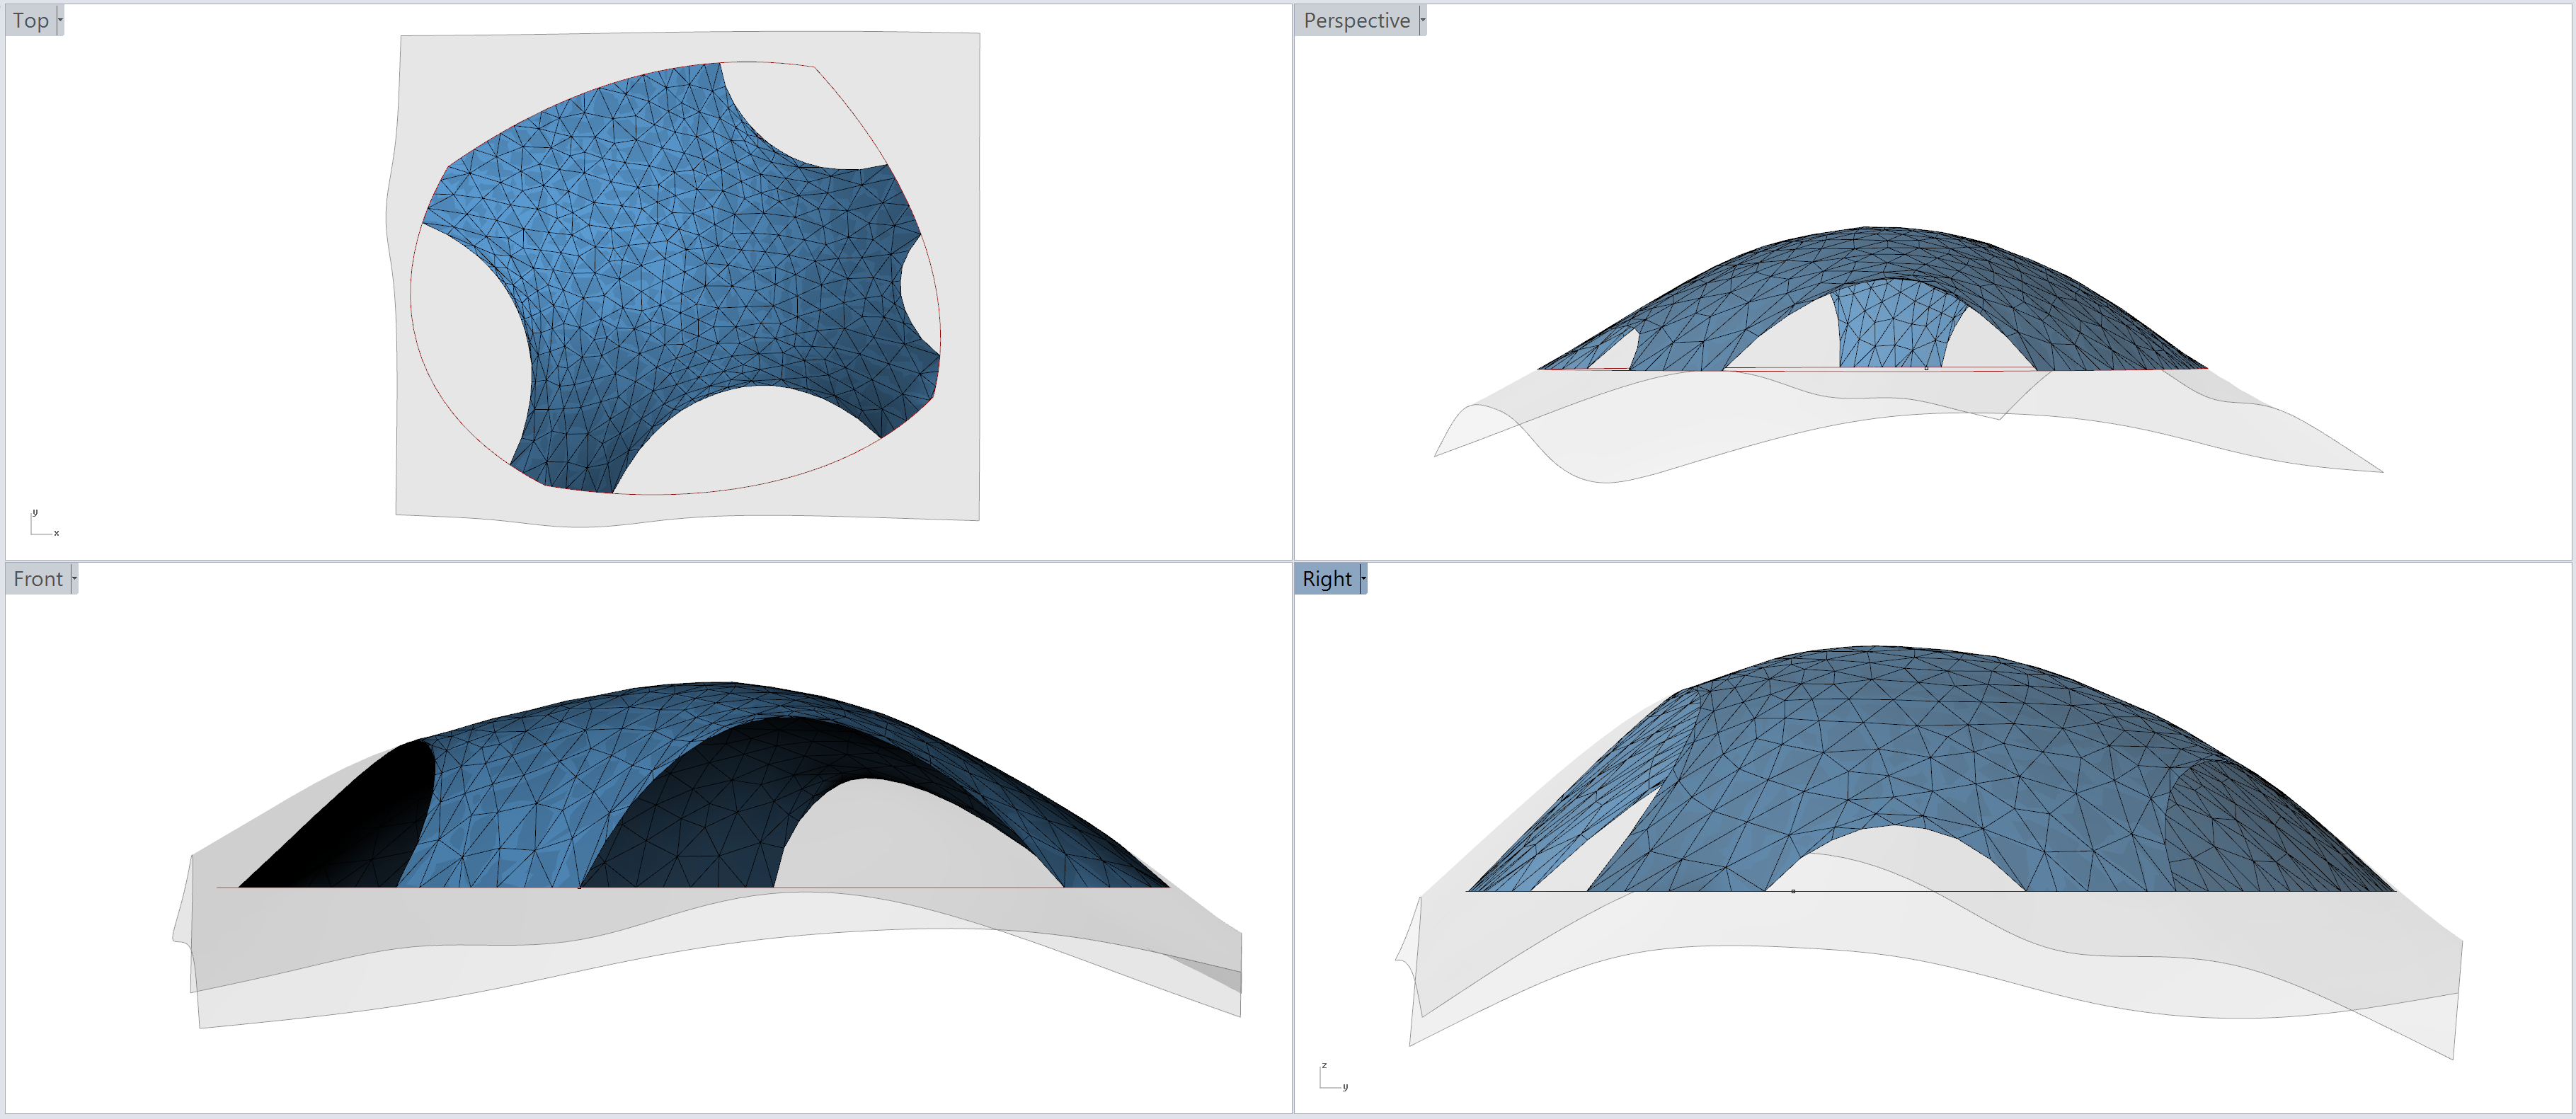
\includegraphics[width=1.0\linewidth ]{figure/Results/surfaMesh.png}
\caption{output from Geodesic}
\end{figure}

Transforming the mesh to a surface is not uncomplicated. The surface did have small deviations from the surface. To give a measure of how much the following metric was used. The average length of the mesh edges gets to resemble average panel, in this case, $4,16 \quad units$. The average distance to the surface was $0.025 \quad units$. One corner that has deviated $0.025 \quad units$ results in an angle of  $0.34$ degrees.

\begin{figure}[H]
\centering
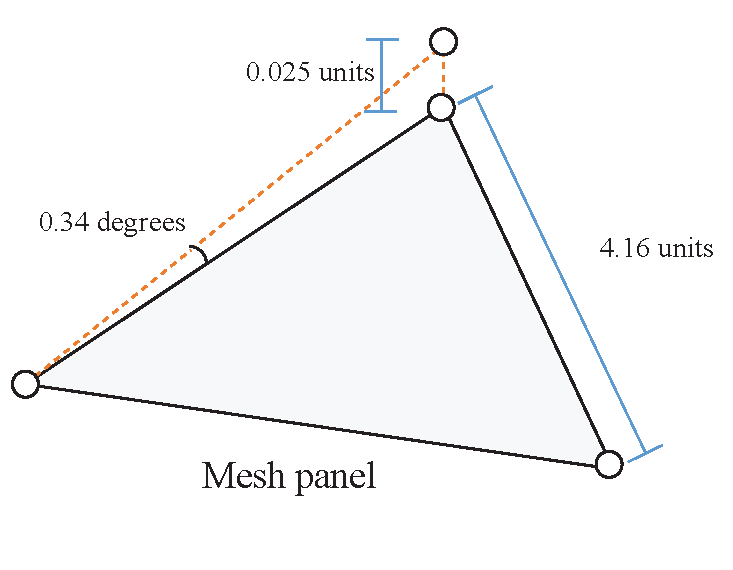
\includegraphics[width=0.7\linewidth ]{figure/Results/devianceSurf.pdf}
\caption{output from Geodesic}
\end{figure}




